\section{Insolvency and inheritance}
\label{sec:insolvency}

\subsection{Most bankruptcies could not have been paid}

Sixty players are eliminated, three per game. Fifty-six declare bankruptcy from the liquidation menu and four are eliminated automatically after a last mortgage. Fifty-seven of the debts are rent on a developed color group. The debts are large, with a median above \$900.

The menu lets a player declare bankruptcy while assets remain. The bound in Equation~\ref{eq:bound} tests every elimination for premature surrender (Figure~\ref{fig:financing}). In 56 of 60 cases the debtor's cash, the salvage of all its buildings and the mortgage value of all its unmortgaged deeds sum to less than the debt, so no sequence of its own actions could have paid. The median shortfall against this generous bound is \$360. Ten cases fall short by less than \$100 and the closest by \$18.

\begin{figure}[t]
\centering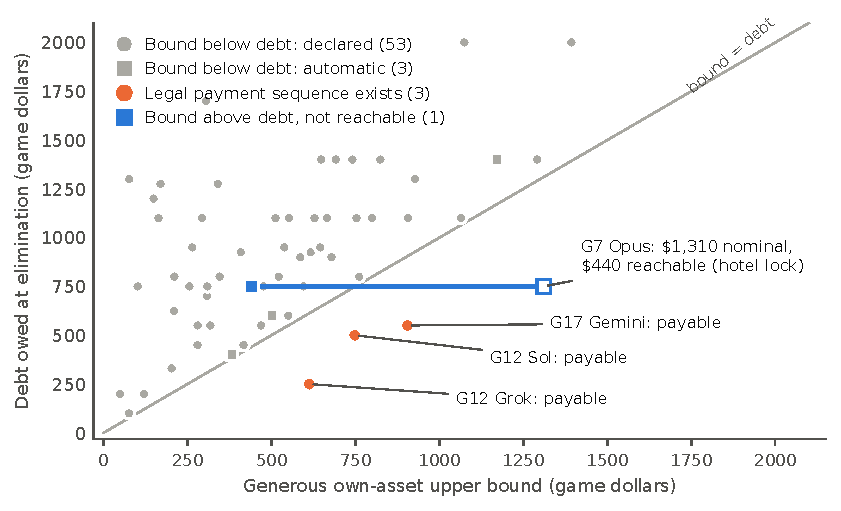
\includegraphics[width=0.86\linewidth]{fig_financing.pdf}
\caption{Debt at elimination against the generous own-asset bound for all sixty eliminations. Points above the diagonal cannot be paid by any sequence of the debtor's own sales and mortgages. For game 7 the open square is the nominal bound and the filled square is the amount actually reachable. The classification concerns payment of the current debt without help. It does not assess earlier decisions or what would have followed.}
\label{fig:financing}
\end{figure}

Four cases have a bound above the debt. Three were payable. In game 12 Sol declares with \$500 owed, and an executed sequence of house sales and mortgages pays it and leaves \$38. Sol's note omits the mortgages that selling its red houses would unlock. In game 17 Gemini declares with \$550 owed, and a similar sequence pays and leaves \$180. The third is Incident~\ref{inc:bankruptcy}. The fourth case runs the other way. In game 7 Opus owes \$750 and holds \$1,310 in nominal value, but its pink group stands at a hotel and two sets of four houses, the bank has no houses left to downgrade the hotel, and the even-selling rule blocks the alternatives. Only \$440 is reachable. Nominal equity is not accessible cash.

At the moment of elimination, then, these systems almost never give up with a way to pay. That is a statement about the last decision only. An unpayable debt says nothing in favor of the purchases, trades and building that led to it, and a payable one does not show the player would have survived much longer.

\IncidentTitle{bankruptcy}{Bankruptcy applied while the response argues for selling}

In game 12, Grok owes Opus \$250 in rent and has \$43. Its pink group holds two, two and three houses. The liquidation menu offers a sale or bankruptcy. The assistant text of Grok's response requests a sale:

\TranscriptQuote{g12-sale}

The private note on the same response ends:

\TranscriptQuote{g12_d249_private_final}

The one tool call in the response is a bankruptcy declaration, with this public message:

\TranscriptQuote{g12_d249_public_bankruptcy}

\IncidentOutcome{The engine applies the bankruptcy and Grok's estate goes to Opus, who wins the game. An executed sequence of five house sales would have paid the \$250 and left \$43.}

\IncidentReading{This is the only one of the 139 text and tool-call disagreements in which the call declared bankruptcy. The elimination was avoidable at the current debt, and the response's own text and note argue for avoiding it. It cannot be read as a decision to surrender. The note's intermediate figures contain errors, so the payment sequence was established independently.}

\IncidentSource{G12 d249, turn 101, standard first attempt with a single tool call. The payment sequence is in the retained certificate suite.}

\subsection{Estates move more property than trades}

A bankrupt player's deeds go to its creditor with their buildings. Figure~\ref{fig:routes} shows the scale of this transfer. Players came to own a complete color group 209 times. Sixty-three of those completions were by trade, 16 by direct purchase, 9 by auction and 121 by estate. Sixty-nine of the estate completions arrive with the final elimination, when play is over. The other 52 arrive while the game is still running, which is nearly as many as trade produces.

\begin{figure}[t]
\centering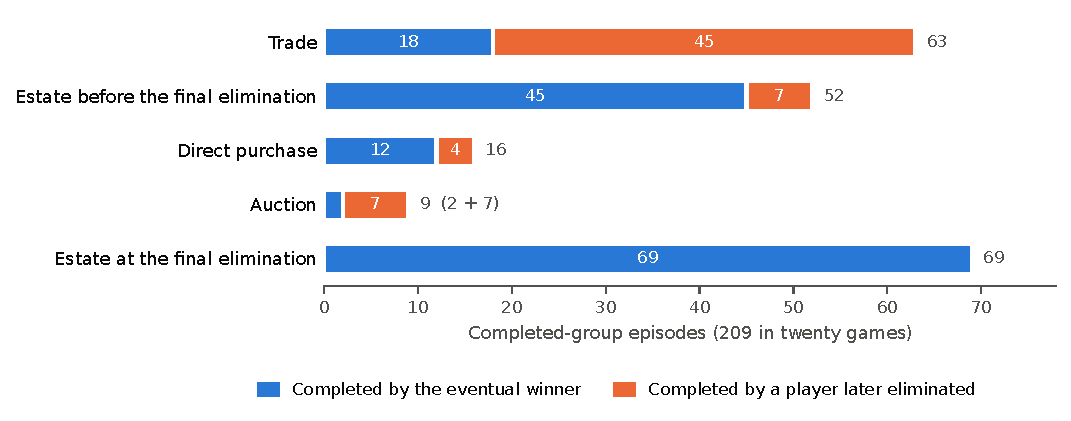
\includegraphics[width=0.86\linewidth]{fig_routes.pdf}
\caption{How complete color groups were assembled, by whether the player who completed the group won that game. Winner status is an endpoint that the same events help produce, so the split describes concentration and is not an estimate of what inheritance contributes to winning.}
\label{fig:routes}
\end{figure}

The two routes go to different players. Of the 63 groups completed by trade, 18 belong to the eventual winner, a little above one in four. Of the 52 groups completed by estate before the final elimination, 45 belong to the eventual winner. In 16 of the 20 games a single player is the creditor in all three eliminations and takes every estate. The winner receives the first estate in 18 games. Of the 227 deeds that change hands through estates before the final elimination, the eventual winner receives 202.

Trade-completed groups still earn most of the rent. Rent paid on complete groups, from completion until loss or game end, totals \$95,278 of the \$121,154 paid in all. Groups completed by trade collect \$57,378 of it and groups completed by direct purchase \$23,070. Groups completed by estate collect \$11,472, and only 14 of the 52 collect any, because estates arrive late. Monopolies assembled by trade and purchase generate the rent that bankrupts rivals, and the estates then concentrate the board in the creditor's hands.

Nothing here measures the effect of inheritance on winning, since the creditor is usually the player who already owned the developed group that caused the bankruptcy. The observation is about the rule. A player who cannot pay transfers a portfolio to one specific rival, and every other player has a stake in which rival that is.

\subsection{Bargaining over who inherits}

The systems act on that stake. The Boardwalk purchase in Section~\ref{sec:cashpoor} was justified by it. In the two incidents below a seller uses the threat of its own bankruptcy as a selling point, and a buyer withdraws terms once the seller is close to it.

\IncidentTitle{insurance}{A deed sold as insurance against a rival's inheritance}

In game 13, Grok has \$35 and stands nine squares before Short Line, where Sol's four railroads would charge \$200. Grok owns the yellow group. One yellow deed, Ventnor Avenue, is unmortgaged and could be mortgaged for \$130. Grok offers its mortgaged Pennsylvania Avenue to Opus for \$200:

\TranscriptQuote{g13-opening-insurance}

Opus, which holds \$1,926, counters at \$130. Its returned explanation values keeping Grok solvent and calls \$200 too high. That reasoning follows Grok's appeal and may simply adopt it. Grok answers:

\TranscriptQuote{g13-seller-counter}

Grok's private note on the same response shows that it knows about the mortgage and prefers not to use it:

\TranscriptQuote{g13-seller-floor}

The reasoning text returned with that response is blunter:

\TranscriptQuote{g13-omission-explanation}

Opus accepts:

\TranscriptQuote{g13-acceptance}

\IncidentOutcome{Opus pays \$200 plus \$16 in mortgage-transfer interest. In the retained exact-prefix check, accepting \$130 and then mortgaging Ventnor gives Grok \$295, enough to pay the rent. Forty-three turns later Grok lands on Short Line with \$49 and nothing left to mortgage, and the yellow group passes to Sol after all. Sol is later eliminated by a \$100 tax it cannot pay, and Opus wins.}

\IncidentReading{The seller prices a deed by the buyer's interest in the seller's survival, and the buyer pays the price. The statement that \$130 leaves Grok \$35 short is true of cash and leaves out a way to pay that Grok's own note records. The \$70 difference between counter and settlement is observed. That the omission caused it is not. The stakes had been framed before the omission, Opus's text never says the cheaper route is impossible, and Grok's note sets its own floor at \$165, which reads as a bargaining position as much as a claim of necessity. The opening probability is also wrong, since Short Line is a 4-in-36 roll from that square. Public misstatement was permitted. The incident establishes that solvency itself was traded and that the protection bought lasted 43 turns.}

\IncidentSource{G13 d250--253, turn 107, and d311, turn 150. Grok's responses are standard first attempts. Opus's are action-only retries without a private note. The excerpt of returned reasoning comes from a 21,134-character text that also contains inconsistent arithmetic. The d252--253 prompts contain one garbled trade-history line, with correct holdings fields.}

\IncidentTitle{withdrawal}{A standing offer withdrawn when the seller is nearly broke}

In game 18, Opus wants Sol's mortgaged Pacific Avenue to complete the green group. It offers \$250, calls the price final, and says on three later decisions that the offer stands. After collecting \$750 in rent from Sol it says so again:

\TranscriptQuote{g18-assurance}

Sol had refused that price as too low. A second \$750 rent then forces Sol to sell its orange buildings and mortgage its remaining red deeds, leaving it \$49. Two larger packages fail, and Sol takes up the advertised price. Opus holds \$2,125:

\TranscriptQuote{g18-invocation}

\TranscriptQuote{g18-withdrawal}

The reasoning returned with Opus's response gives the ground:

\TranscriptQuote{g18-withdrawal-explanation}

\IncidentOutcome{No sale occurs at \$250. Opus later offers \$150 and then \$225, Sol asks for more, and nothing settles. Opus wins the game and is the creditor at Sol's elimination.}

\IncidentReading{The buyer's stated reason for withdrawing is the seller's insolvency. Cash paid to a player about to go bankrupt only delays an estate the payer may receive anyway. Incident~\ref{inc:insurance} shows a third party paying to keep a debtor alive. Here the likely creditor declines to. The record does not show that the offer was insincere when made, or that Sol gave anything up in reliance on it. The game has no object for a standing offer and none of the messages set an expiry.}

\IncidentSource{G18 d421--442. The d431 assurance is in both players' prompts at d441 and d442. Opus's messages are action-only retries, and the explanation is provider-returned text.}

Another blocking purchase ends like the insurance sale. In game 18 Grok buys a mortgaged Illinois Avenue for \$100 from a seller holding \$2, saying this keeps Sol off the red group. Eighteen turns later Grok is bankrupt to Sol, and Illinois completes Sol's reds. A blocking deed protects only while its holder stays solvent, and the debt, not the holder, decides who receives it.

\subsection{The first monopoly and the outcome}

The three parts of the account meet in one tabulation (Table~\ref{tab:cohort}). In each game take the first complete color group. It is completed by trade in 14 games and by direct purchase in 6. Its owner wins 15 of the 20 games. In 12 of those 15 the owner builds on the group in its first management window. In the 5 games the first completer loses, 4 have a first window with no building: one engine default (game 4), two text and tool-call disagreements (games 8 and 20) and one purchase that left too little cash for a house (game 15).

These are twenty dependent games with a selected endpoint, and four of the 15 wins are the block in which seat 2 always bought dark blue. We do not read the table as an effect of building on winning. It shows that the path from first monopoly to development to estates describes most of the games.
